%!TEX root = ../../main.tex

\chapter{Item collections}
\index{Item collection}

\section{Empty content indicator}
\label{sec:empty_content_indicator}

\index{Layout content!Empty content}
\index{Item collection!Empty content}

If one should have that the content is a dynamic collection of items and that collection is empty one should indicate that there are no items avaiable. This indicator should be a text with a gray text-color (\colref{1.2}) like seen in \figref{fig:empty_content_noitems}.

\begin{figure}
    \centering
    \begin{subfigure}[t]{0.4\textwidth}
        \centering
        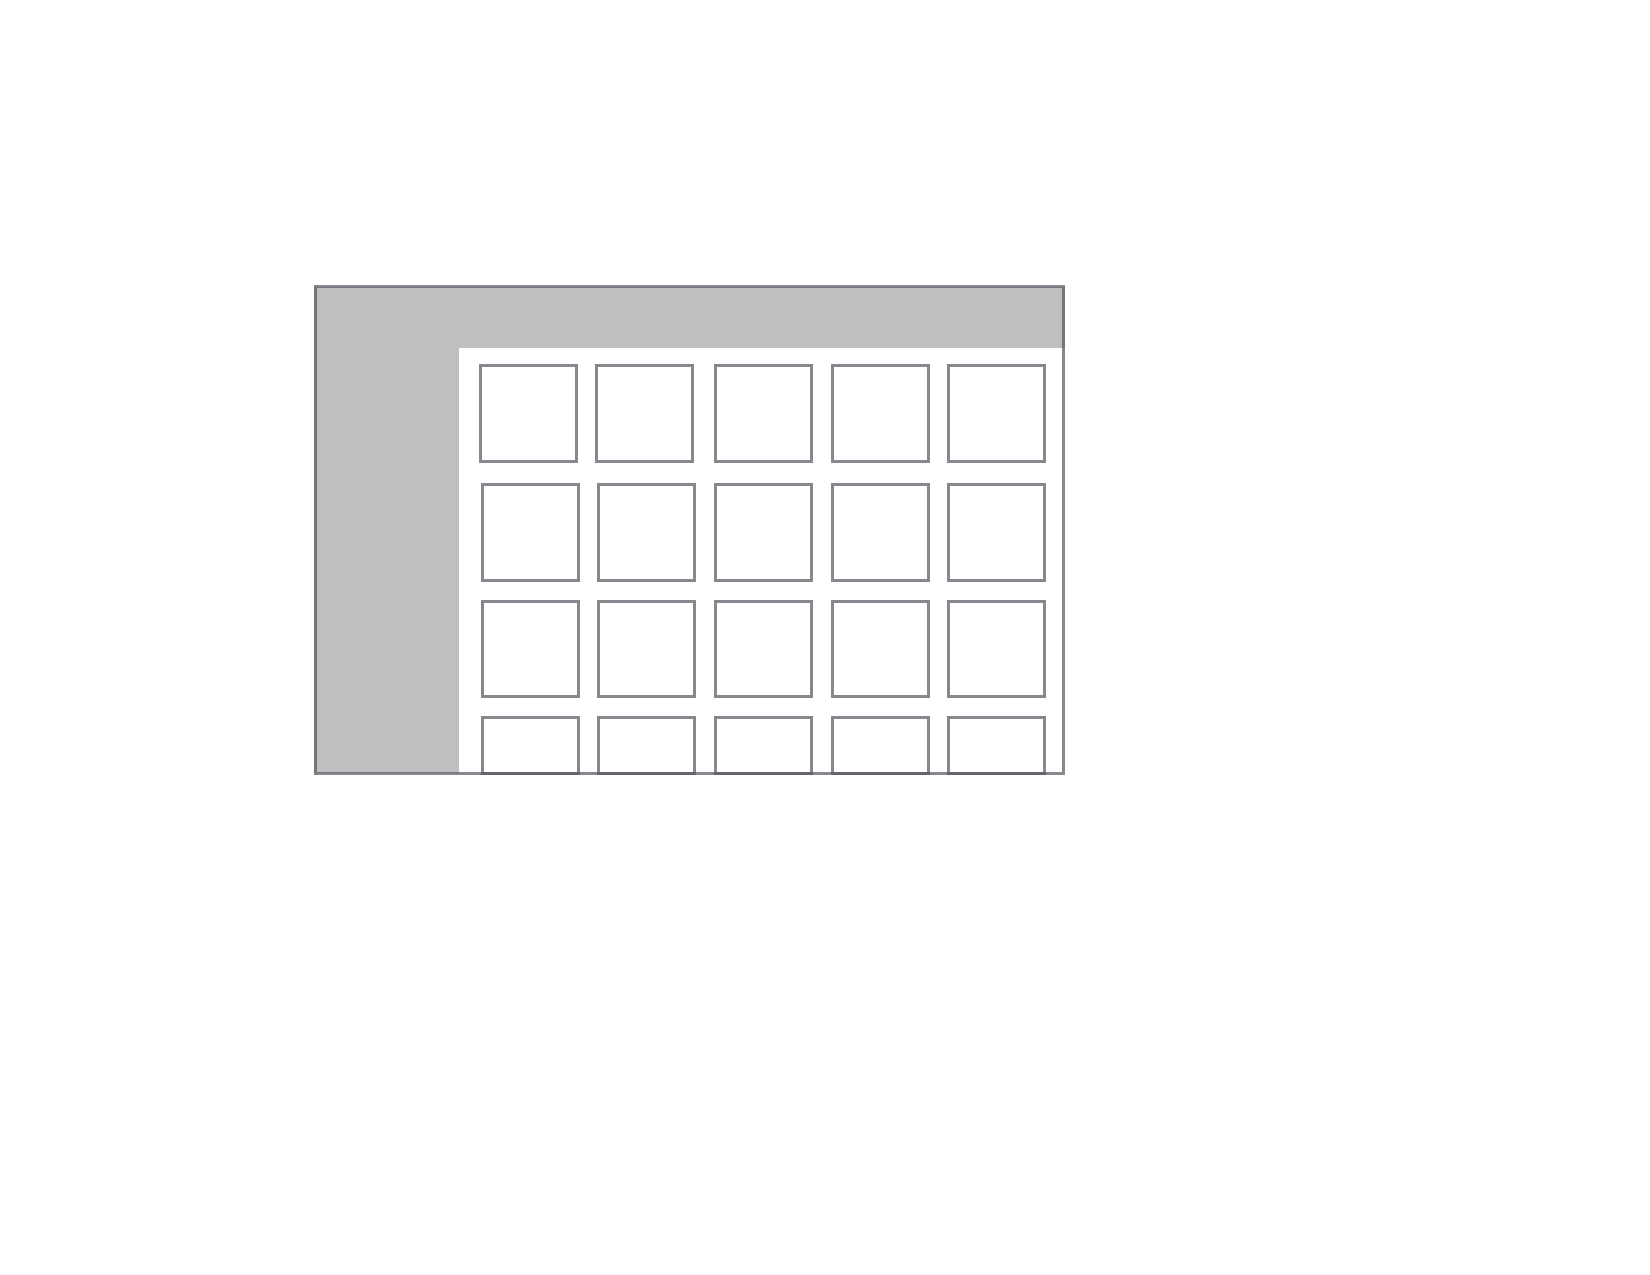
\includegraphics[scale=0.4]{item_collection_items}
        \caption{Content with items}
        \label{fig:empty_content_items}
    \end{subfigure}
    \hspace{5em} 
    \begin{subfigure}[t]{0.4\textwidth}
        \centering
        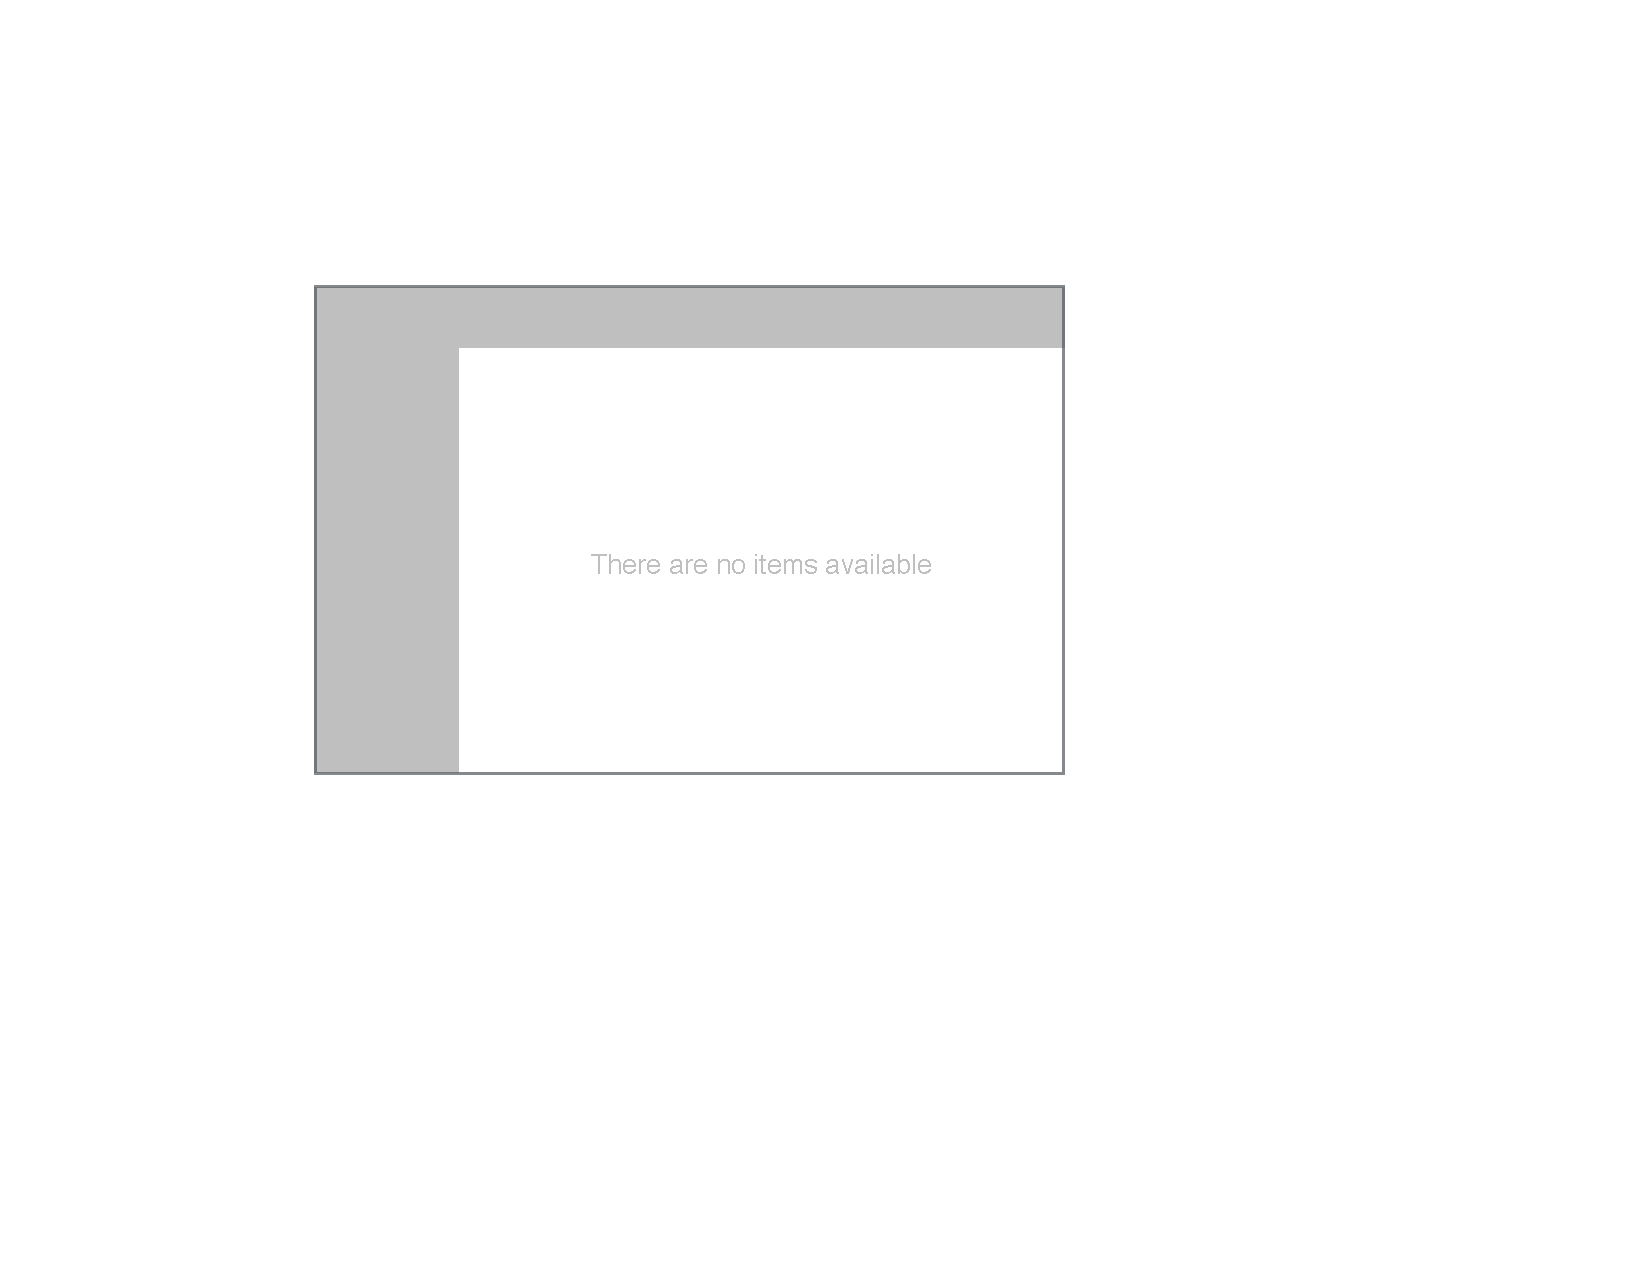
\includegraphics[scale=0.4]{item_collection_noitems}
        \caption{Content with no items}
        \label{fig:empty_content_noitems}
    \end{subfigure}
    
    \caption{Empty content indicator}
    \label{fig:empty_content}
\end{figure}

\FloatBarrier

\section{Overscroll}
\label{sec:overscroll}

When a view has a collection of items and the user tried to scroll further than there are elements a gray shadow should be display as seen in \figref{fig:overscroll}.

\begin{figure}[h]
    \centering
    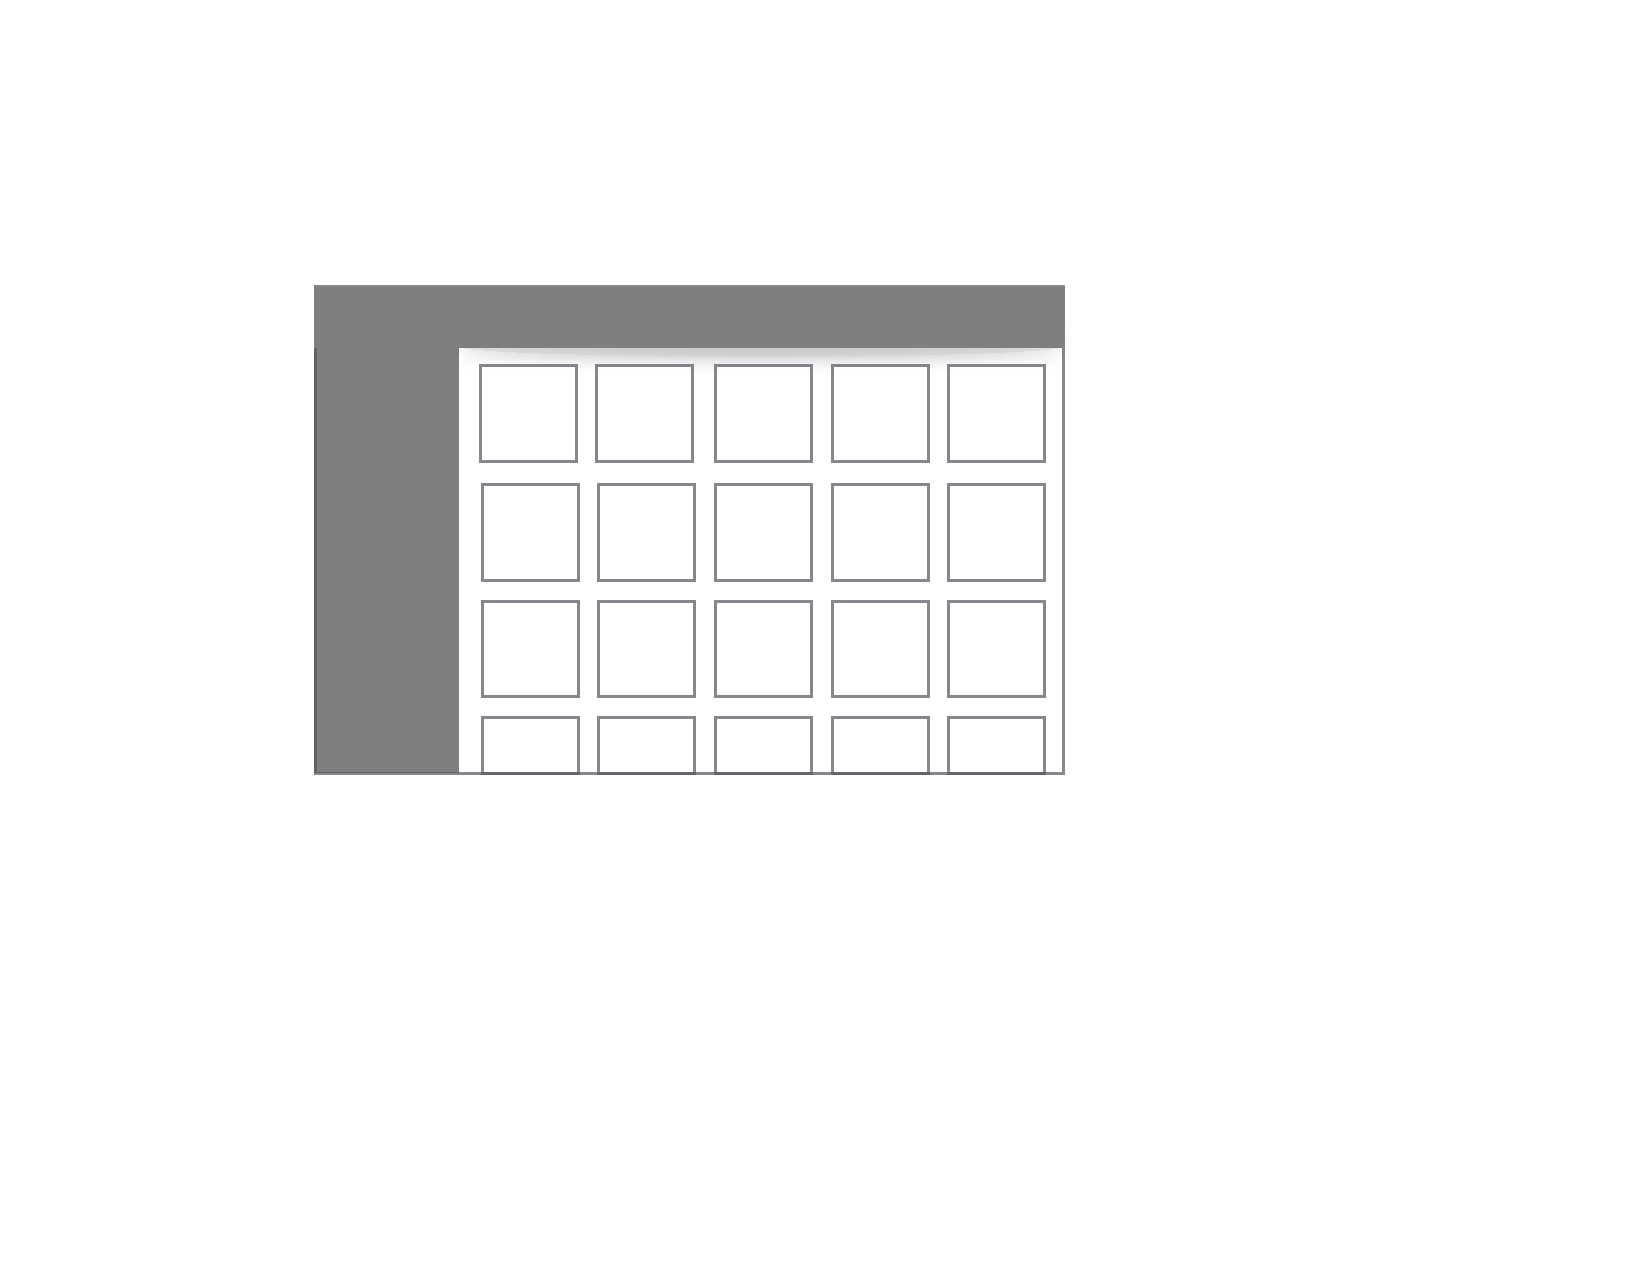
\includegraphics[scale=0.5]{overscroll_shadow}
    \caption{Content with overscroll shown in top}
    \label{fig:overscroll}
\end{figure}

\FloatBarrier

\section{Updates in the collection}
\label{sec:updates_in_the_collection}

When updating a collection of items one should notify the user that some change in the collection have happend. There are two legal ways to this:
\begin{enumerate}
    \item Add the item as the first element in the collection as seen in \figref{fig:item_collection_after_update_one}.
    \item Move the view of the collection to place where the item is added as seen in \figref{fig:item_collection_after_update_two}.
\end{enumerate}

\begin{figure}[htbp]
    \centering
    \begin{subfigure}[t]{0.2\textwidth}
        \centering
        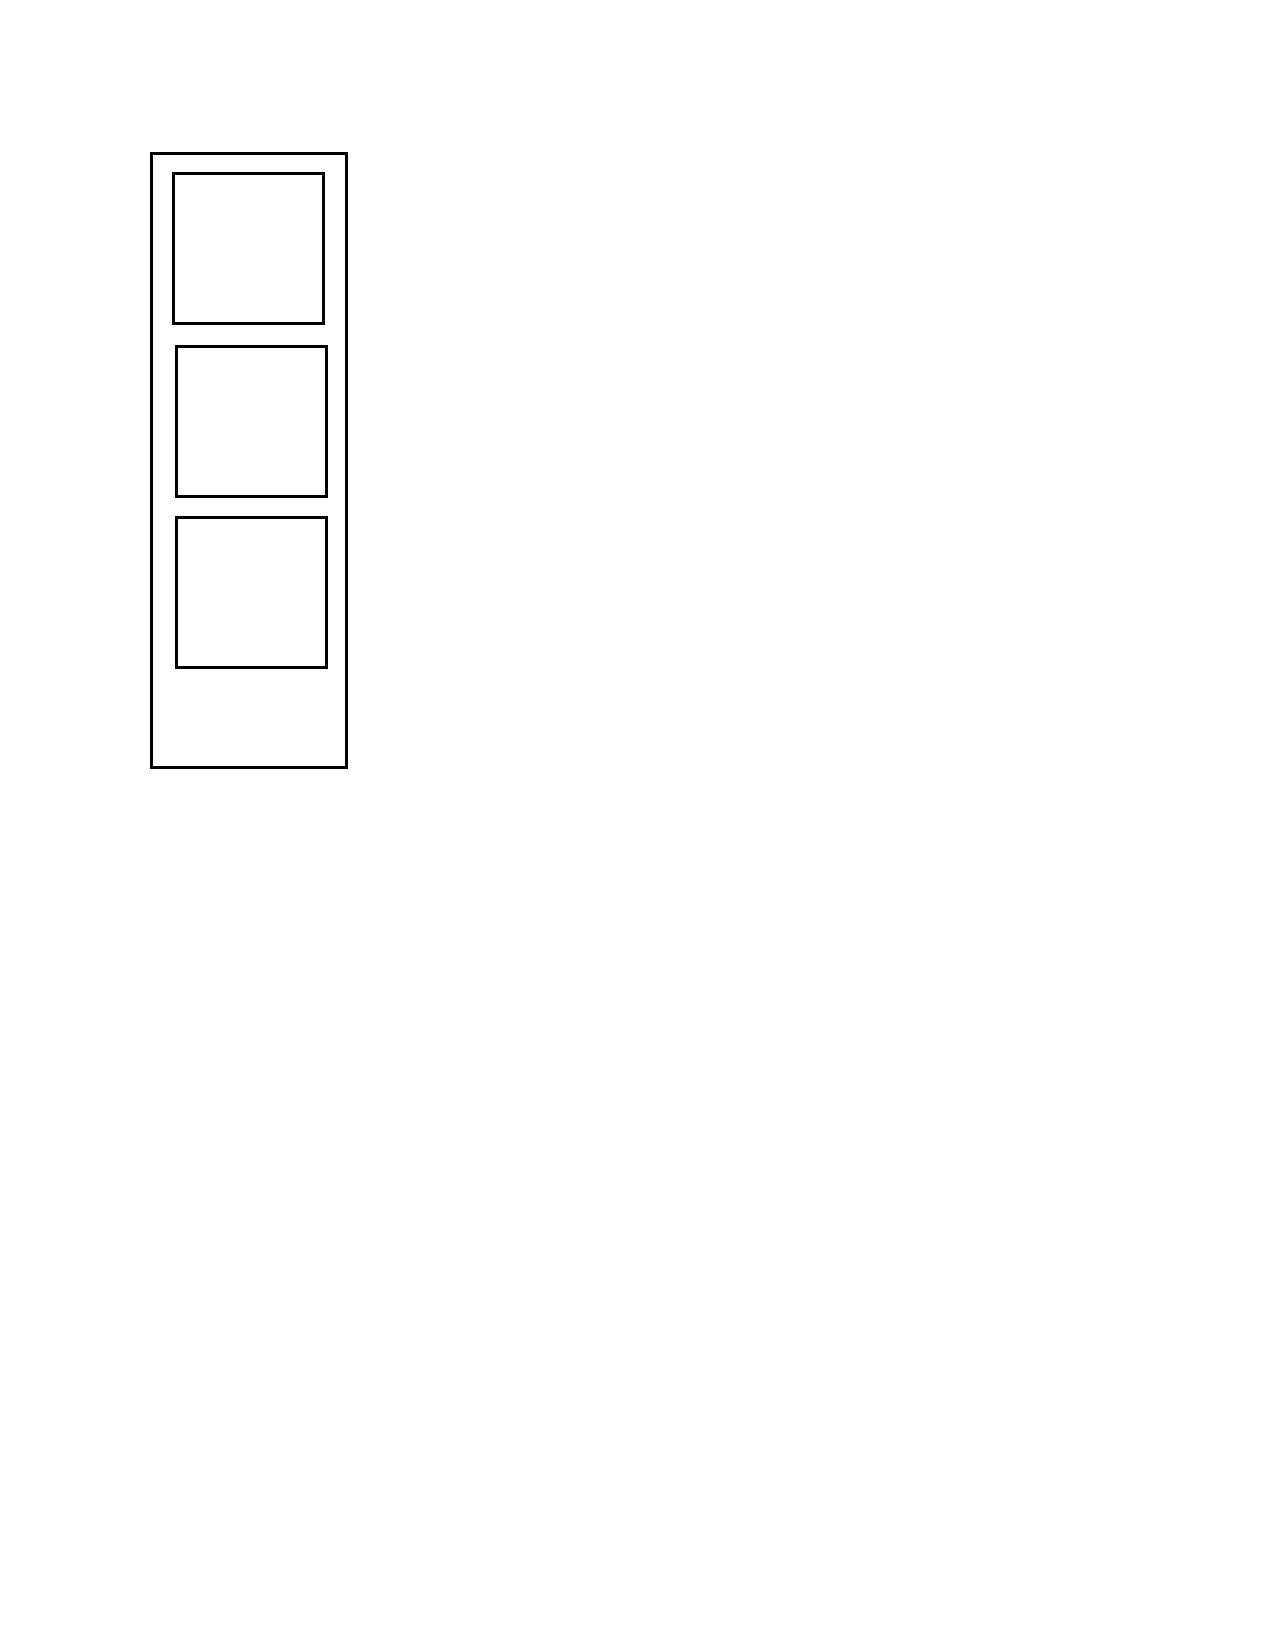
\includegraphics[scale=0.6]{item_collection_update/item_collection_before_update}
        \caption{Item collection before udpate}
        \label{fig:item_collection_before_update}
    \end{subfigure}
    \hspace{2em} 
    \begin{subfigure}[t]{0.2\textwidth}
        \centering
        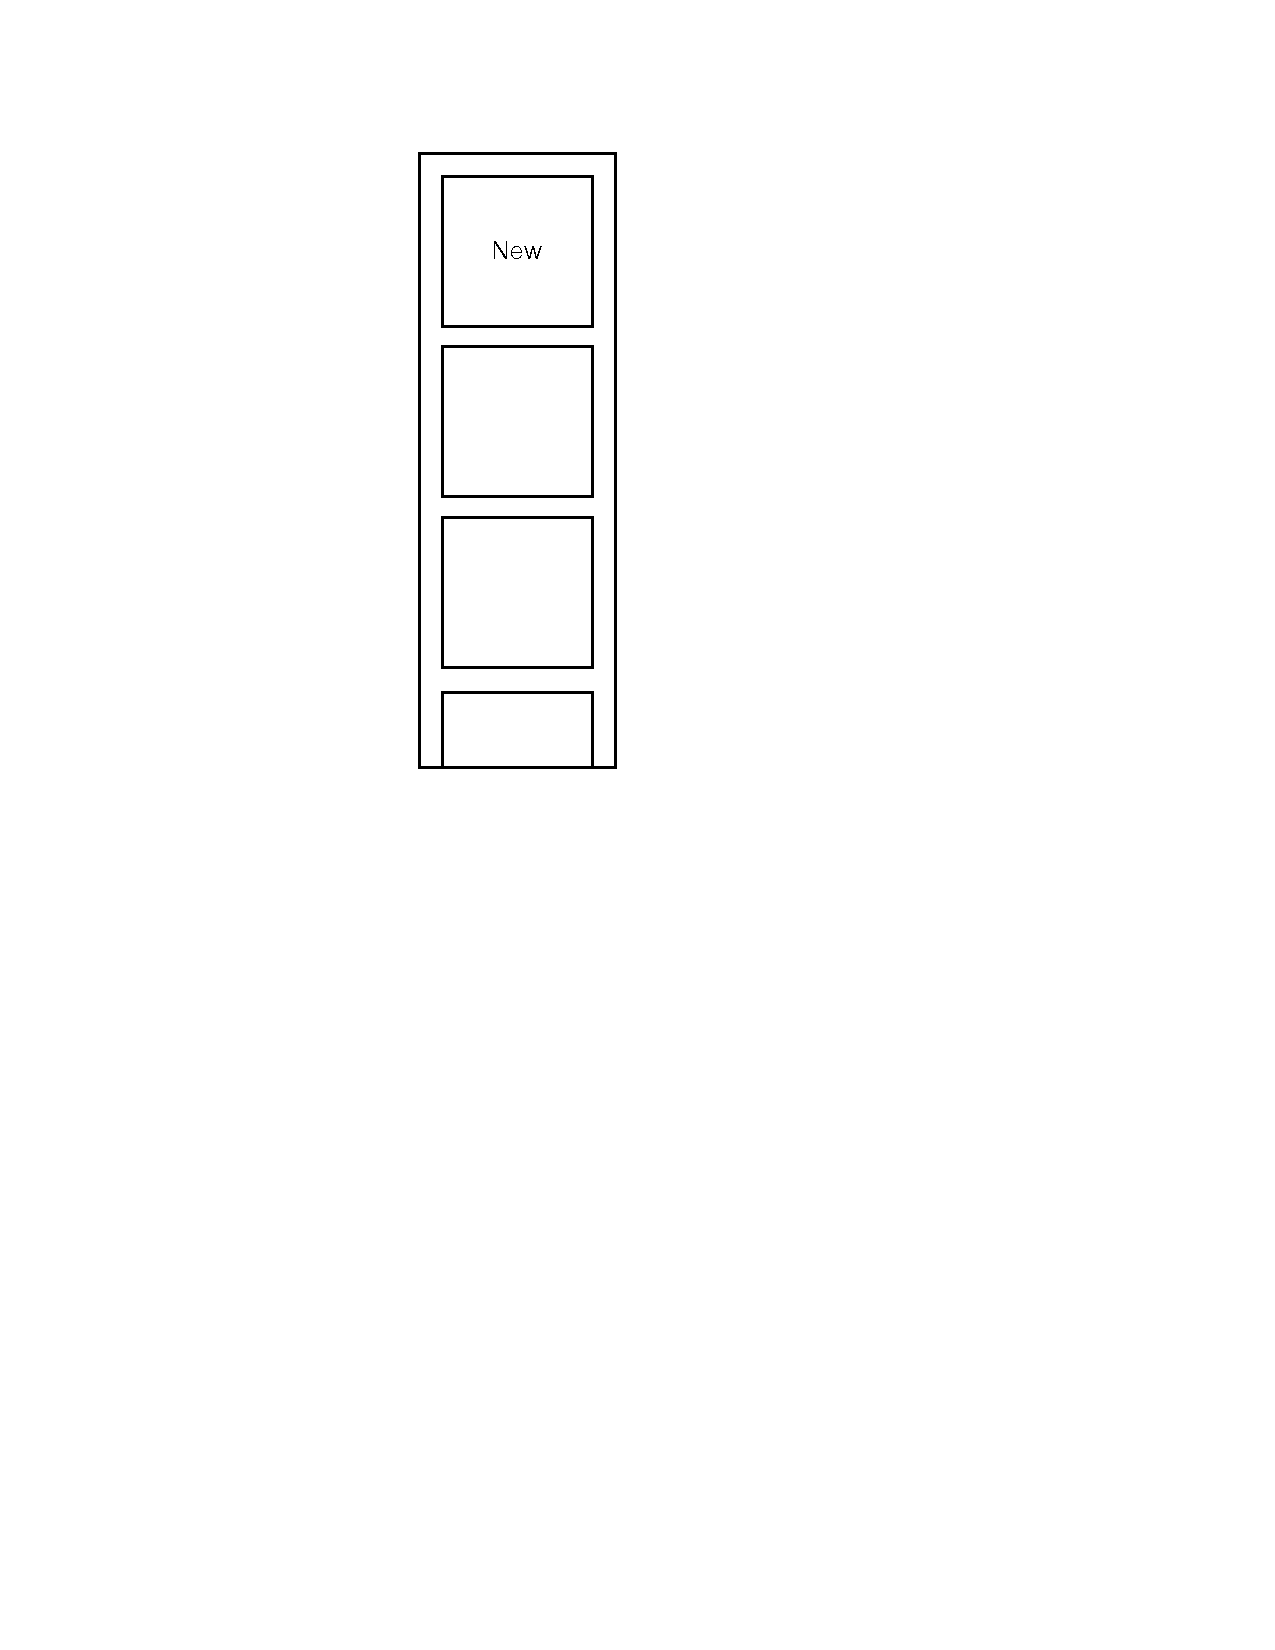
\includegraphics[scale=0.6]{item_collection_update/item_collection_after_update_one}
        \caption{Item collection afer udpate option \#1}
        \label{fig:item_collection_after_update_one}
    \end{subfigure}
    \hspace{2em} 
    \begin{subfigure}[t]{0.2\textwidth}
        \centering
        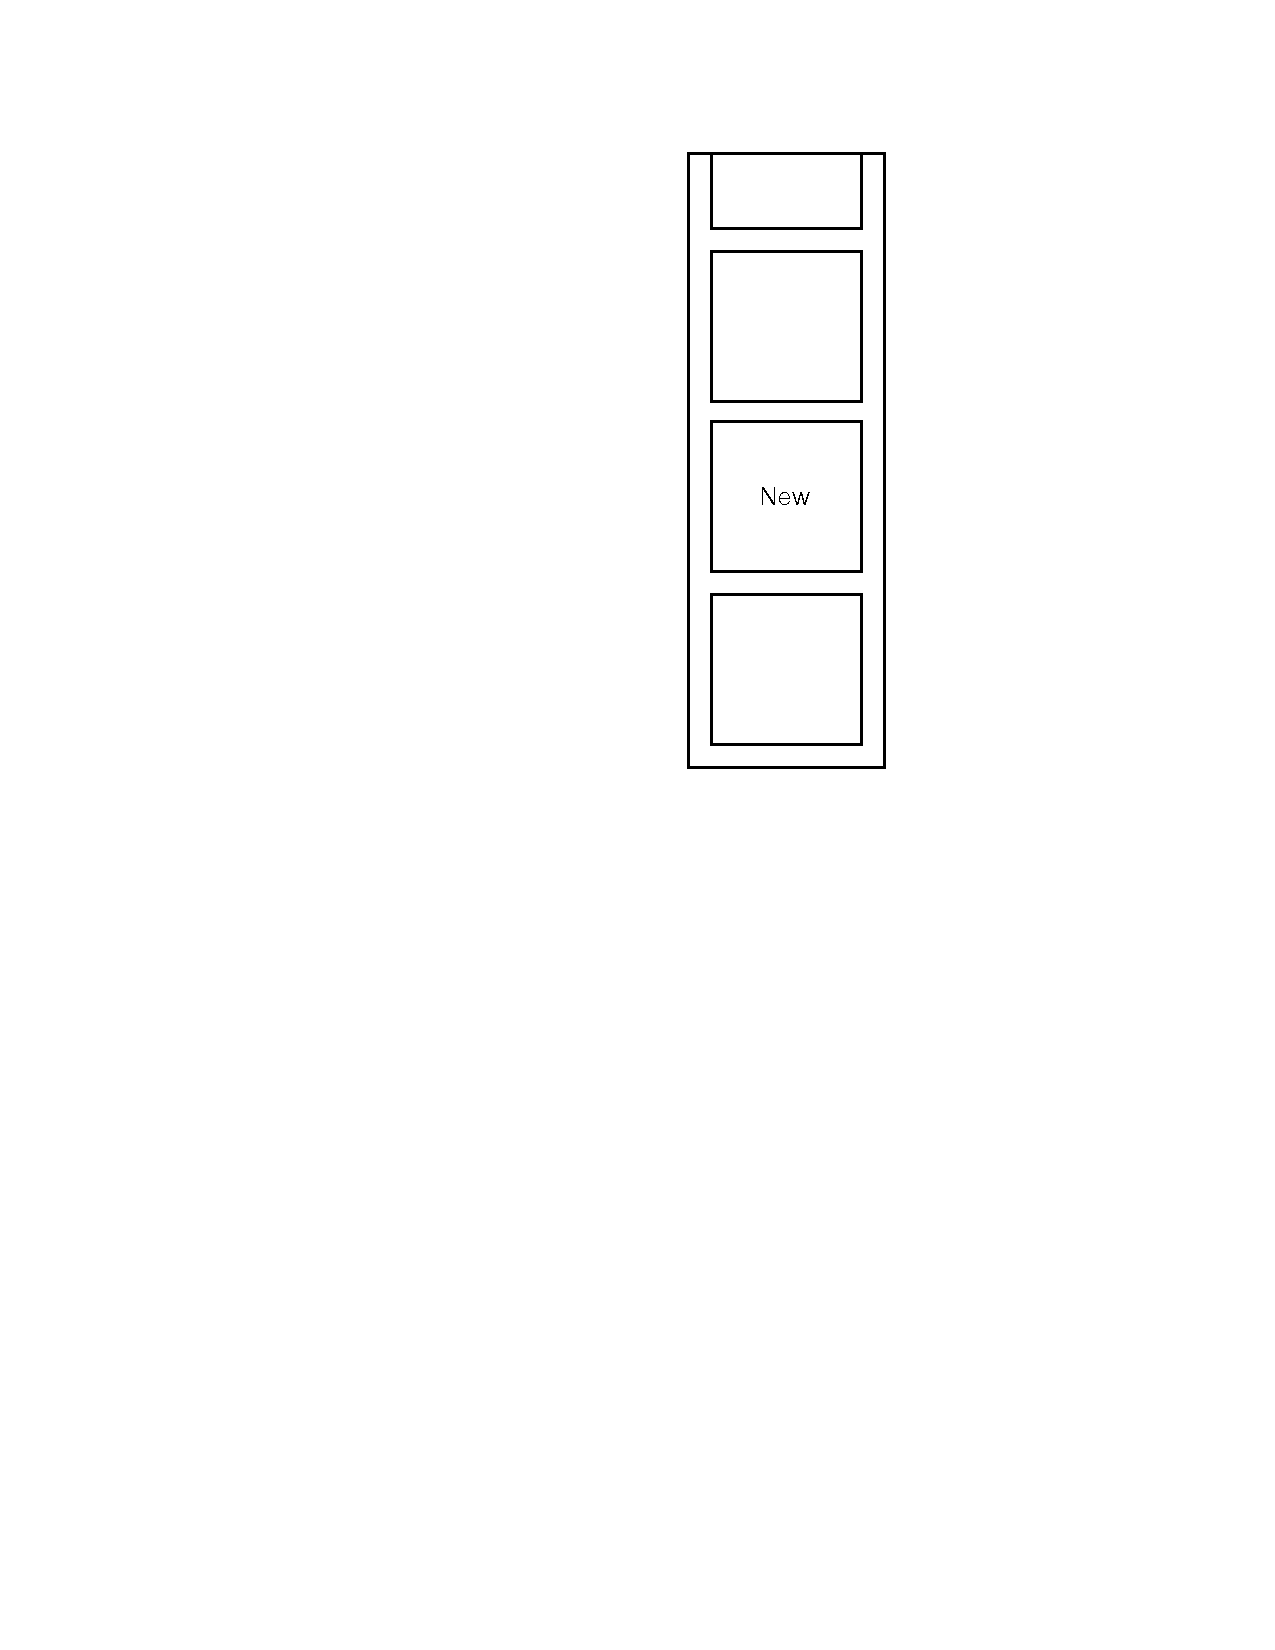
\includegraphics[scale=0.6]{item_collection_update/item_collection_after_update_two}
        \caption{Item collection after udpate option \#2}
        \label{fig:item_collection_after_update_two}
    \end{subfigure}
    \hspace{2em} 
    \begin{subfigure}[t]{0.2\textwidth}
        \centering
        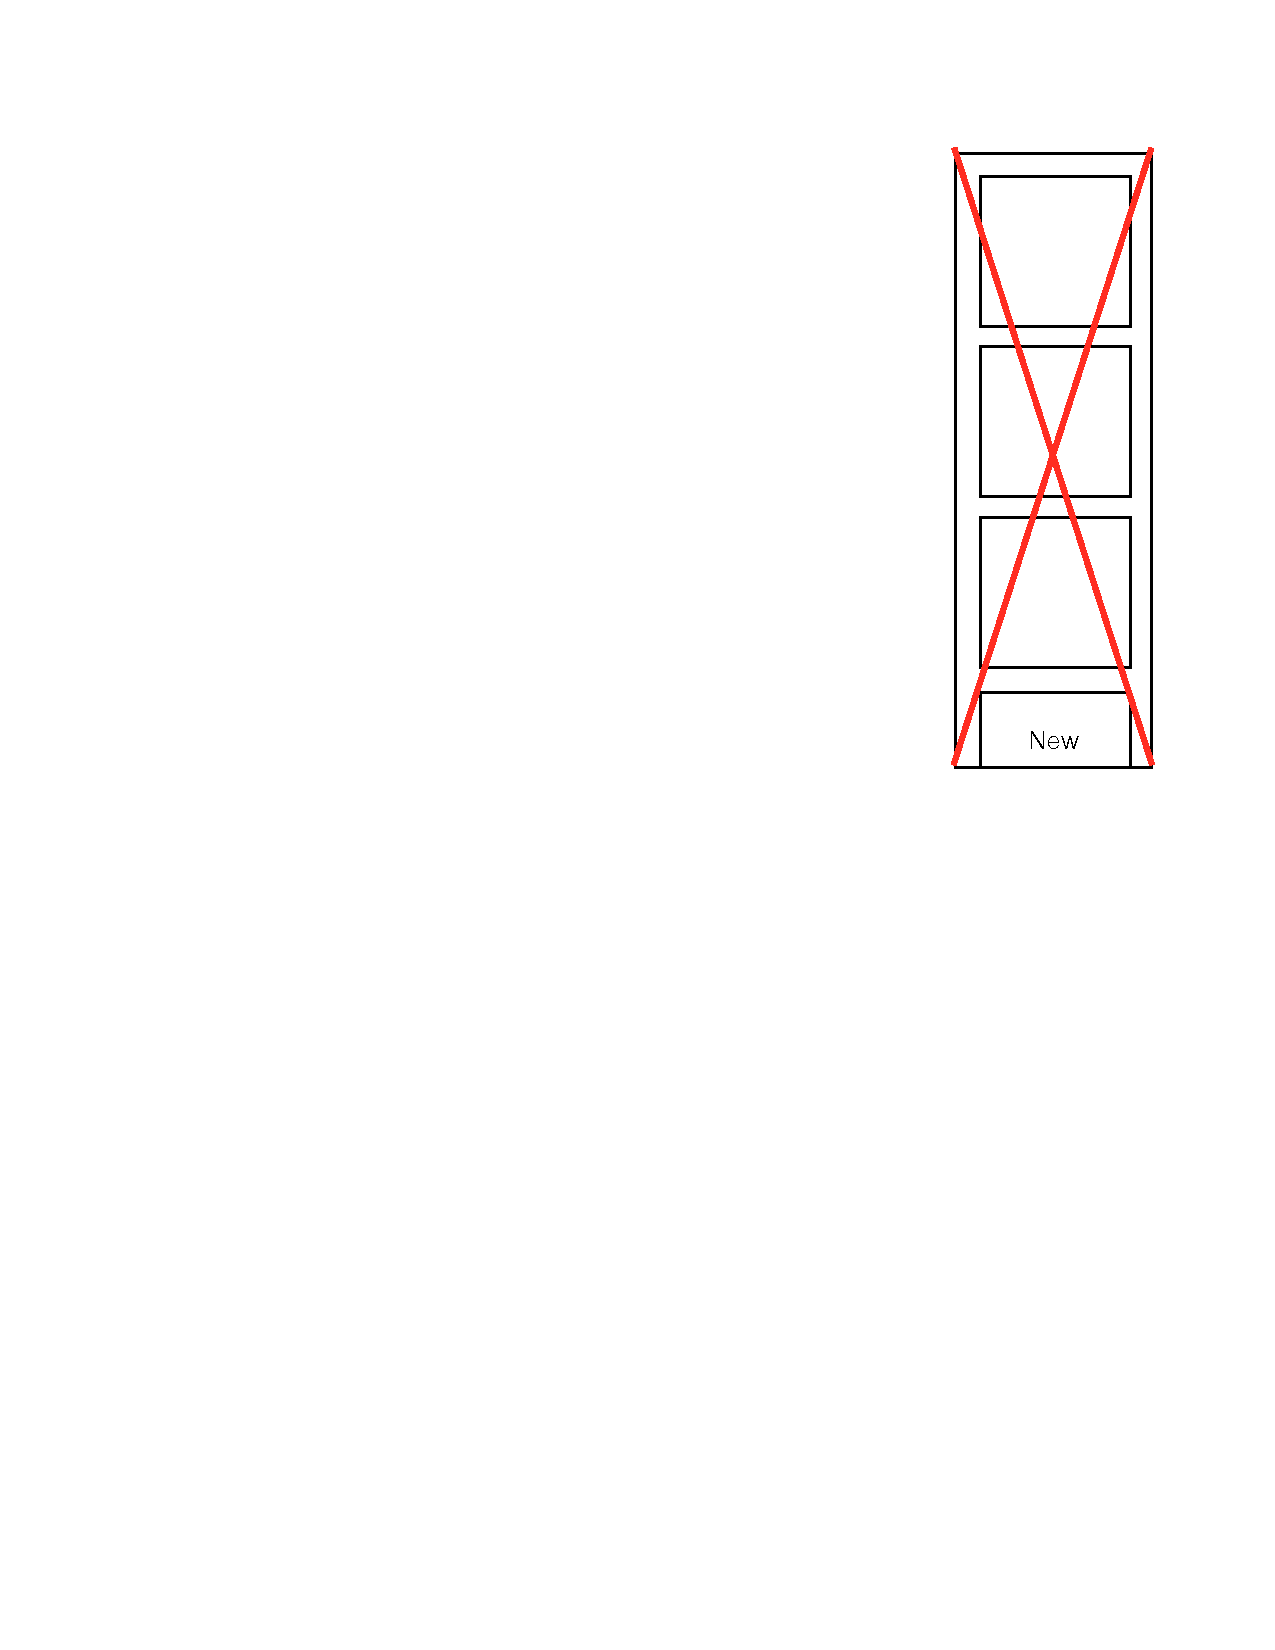
\includegraphics[scale=0.6]{item_collection_update/item_collection_after_update_wrong}
        \caption{Wrong item collection af udpate}
        \label{fig:item_collection_after_update_wrong}
    \end{subfigure}
    
    \caption{Update of item collection}
    \label{fig:item_collection_update}
\end{figure}

\FloatBarrier

\section{Reordering in the collection}
\label{sec:reordering_in_the_collection}

\todo[inline]{Describe how one may reorder in a collection of items. For isntance the bottombar in the Pictoreader}